\section{Introduction}


\subsection{Summarization}

\begin{frame}{Summarization Overview}

	\begin{itemize}
		\item \textbf{Definition} Summarization involves condensing natural language
		while retaining essential information for quicker readability and interpretation.
		\item \textbf{Importance} Summarization is crucial because it helps us extract
		important information efficiently.
		\item \textbf{Role for long texts} Summarization can be a valuable tool with
		long texts that can let us decide whether the whole text is worth reading.
	\end{itemize}

	\vskip .5cm

	\begin{figure}
		\centering
		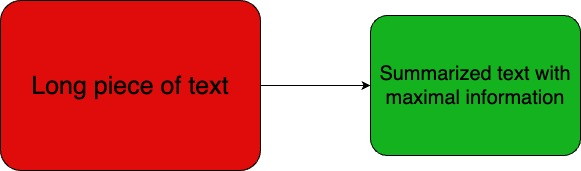
\includegraphics[width=.8\textwidth]{Images/summarize.jpg}
	\end{figure}

\end{frame}


\subsection{Automatic Summarization}

\begin{frame}{What's Automatic Summarization?}

	Summarization done by a computer algorithm automatically is known as automatic
	summarization.

	\vskip .5cm

	\begin{itemize}
		\item \textbf{Extractive methods} Extract key sentences or phrases from the text.
		\item \textbf{Abstractive methods} Generate summary from scratch.
		Higher quality of summary than extractive methods but computationally expensive.
	\end{itemize}

	\vskip .5cm

	\begin{figure}
		\centering
		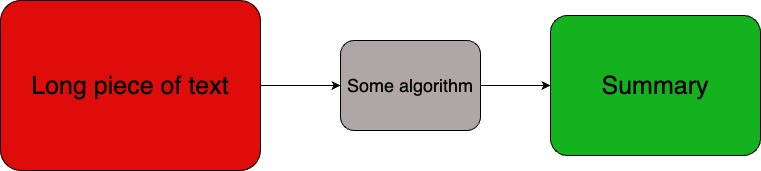
\includegraphics[width=.9\textwidth]{Images/algorithm-summarize.jpg}
	\end{figure}

\end{frame}

\begin{frame}{How is it done today?}

	Nowadays, we have sophisticated Large Language Models (LLMs) based on the
	Transformer architecture \citep{vaswani2017attention} for automatic summarization.
	These methods have pushed the boundaries of abstractive summarization and can
	generate accurate, coherent, and human-like summaries.

	\vskip 1.3cm

	\begin{figure}
		\centering
		
\includegraphics[width=.2\textwidth]{Images/GPT-4.png}
		\hfill
		
\includegraphics[width=.4\textwidth]{Images/bert.jpg}
		\hfill
		
\includegraphics[width=.35\textwidth]{Images/llama.jpg}
	\end{figure}

\end{frame}
